\documentclass[twoside,twocolumn]{article}

\usepackage{blindtext} % Package to generate dummy text throughout this template 
\usepackage{graphicx}
\usepackage[sc]{mathpazo} % Use the Palatino font
\usepackage[T1]{fontenc} % Use 8-bit encoding that has 256 glyphs
\linespread{1.05} % Line spacing - Palatino needs more space between lines
\usepackage{microtype} % Slightly tweak font spacing for aesthetics

\usepackage[english]{babel} % Language hyphenation and typographical rules

\usepackage[hmarginratio=1:1,top=32mm,columnsep=20pt]{geometry} % Document margins
\usepackage[hang, small,labelfont=bf,up,textfont=it,up]{caption} % Custom captions under/above floats in tables or figures
\usepackage{booktabs} % Horizontal rules in tables
\usepackage{graphicx}
\usepackage{lettrine} % The lettrine is the first enlarged letter at the beginning of the text

\usepackage{enumitem} % Customized lists
\setlist[itemize]{noitemsep} % Make itemize lists more compact

\usepackage{abstract} % Allows abstract customization
\renewcommand{\abstractnamefont}{\normalfont\bfseries} % Set the "Abstract" text to bold
\renewcommand{\abstracttextfont}{\normalfont\small\itshape} % Set the abstract itself to small italic text

\usepackage{titlesec} % Allows customization of titles

\titleformat{\section}[block]{\large\scshape\centering}{\thesection.}{1em}{} % Change the look of the section titles
\titleformat{\subsection}[block]{\large}{\thesubsection.}{1em}{} % Change the look of the section titles

\usepackage{fancyhdr} % Headers and footers
\pagestyle{fancy} % All pages have headers and footers
\fancyhead{} % Blank out the default header
\fancyfoot{} % Blank out the default footer
\fancyhead[C]{Comparative Datawarehouse vs Datalake $\bullet$ Abril 2022 $\bullet$ } % Custom header text
\fancyfoot[RO,LE]{\thepage} % Custom footer text

\usepackage{titling} % Customizing the title section

\usepackage{hyperref} % For hyperlinks in the PDF

%----------------------------------------------------------------------------------------
%	TITLE SECTION
%----------------------------------------------------------------------------------------
\providecommand{\keywords}[1]{
  \small	
  \textbf{\textit{\quad \quad Keywords: }} #1}

\providecommand{\pclave}[1]{
  \small	
  \textbf{\textit{\quad \quad Palabras Clave: }} #1}

%Idiomas: \selectlanguage{english} \selectlanguage{spanish}

\begin{document}

\title{Trabajo Encargado 03: Comparative Datawarehouse vs Datalake}

\begin{titlepage}
\begin{figure}[htb]
\begin{center}

\includegraphics[width=5cm]{imagenes/logo.png}
\end{center}
\end{figure}
\vspace*{-0.25in}
\begin{center}
\large{UNIVERSIDAD PRIVADA DE TACNA}\\
\vspace*{-0.025in}
INGENIERIA DE SISTEMAS  \\	

\vspace*{0.5in}
\begin{large}
TITULO:\\
\end{large}

\vspace*{0.1in}
\begin{Large}
\textbf{ Comparative Datawarehouse vs Datalake} \\
\end{Large}

\vspace*{0.3in}
\begin{Large}
\textbf{CURSO:} \\
\end{Large}

\vspace*{0.1in}
\begin{large}
Inteligencia de Negocios\\
\end{large}

\vspace*{0.3in}
\begin{Large}
\textbf{DOCENTE:} \\
\end{Large}

\vspace*{0.1in}
\begin{large}
 Ing. Patrick Cuadros Quiroga\\
\end{large}

\vspace*{0.2in}
\vspace*{0.1in}
\begin{large}

Integrantes: \\
\begin{flushleft}
Maldonado Cancapi, Carlos Alejandro\hfill(2018000660) \\
Huillca Aroni, Alfredo\hfill(2018060903)\\
Anahua Huayhua, Jenny Karen\hfill(2018062150)\\
Coloma Colquehuanca, Kiara\hfill(2018062218)\\

\end{flushleft}
\end{large}

\vspace*{0.1in}
\begin{large}
Tacna - Perú\\
2022
\end{large}
\end{center}
\end{titlepage}

\setlength{\droptitle}{-4\baselineskip} % Move the title up

\pretitle{\begin{center}\Huge\bfseries} % Article title formatting
\posttitle{\end{center}} % Article title closing formatting
\title{Comparative Datawarehouse vs Datalake} % Article title

\date{\today} % Leave empty to omit a date                     
\renewcommand{\maketitlehookd}{%

}

%----------------------------------------------------------------------------------------



% Print the title
\maketitle

%----------------------------------------------------------------------------------------
%	ARTICLE CONTENTS
%----------------------------------------------------------------------------------------

\section{Resumen}
Los datos son el ingrediente más valioso para cualquier organización, desde el procesamiento de grandes volúmenes de datos hasta su almacenamiento y análisis para obtener más información. El almacenamiento de datos es una tarea competitiva cuando hablamos de big data, especialmente por el volumen absoluto de datos involucrados. Dos metodologías populares se centran en el almacenamiento de datos y, a menudo, se comparan entre sí: Data Lake vs Data warehouse.

Ambas terminologías se usan principalmente para Big Data Storage y, por lo tanto, a menudo se usan indistintamente. Pero hay grandes diferencias en lo que ofrecen. Tienen diferentes propósitos y son aplicables a las organizaciones, según los requerimientos. Tienen diferentes estructuras y capacidades de procesamiento y, por lo tanto, tendrán una base de usuarios distinta.


%------------------------------------------------

\section{Abstract}

Data is the most valuable ingredient for any organization, right from processing huge volumes of data to storing them to analyzing them for further insights. Data storage is a competitive task when we talk of big data, especially because of the absolute volume of data involved. Two popular methodologies focus on data storage and are often compared with each other – Data Lake vs Data warehouse.

Both these terminologies are mainly used for Big Data Storage and hence often used interchangeably. But there are major differences in what they offer. They have different purposes and are applicable to organizations, as per requirements. They have different structures and processing capabilities and hence will have a distinct user base.







%------------------------------------------------
\section{Introduccion}
Los Data lakes y Data Warehouse se usan ampliamente para almacenar grandes datos , pero no son términos intercambiables. Un lago de datos es una gran cantidad de datos sin procesar, cuyo propósito aún no está definido. Un almacén de datos es un depósito de datos estructurados y filtrados que ya han sido procesados para un propósito específico. Incluso hay una tendencia emergente de Data lakehouse, que combina la flexibilidad de un lago de datos con las capacidades de gestión de datos de un almacén de datos.
Los dos tipos de almacenamiento de datos a menudo se confunden, pero son mucho más diferentes de lo que se parecen. De hecho, la única similitud real entre ellos es su propósito de alto nivel de almacenamiento de datos.

\begin{center}

\end{center}

\section{Desarrollo}

\subsection{datawarehouse}
\subsubsection{Concepto}
El concepto de data warehouse o almacén de datos se originó en 1988 con el trabajo de los investigadores de IBM, Barry Devlin y Paul Murphy, aunque el término data warehouse fue acuñado por William H. Inmon, el cual es conocido como el padre de Data Warehousing. Inmon describió un almacén de datos como una colección de datos orientada a un tema específico, integrado, variante en el tiempo y no volátil, que soporta el proceso de toma de decisiones. 
Según lo definió el propio Bill Inmon, el Data Warehouse se compone de las siguientes características:
\begin{itemize}
    \item   Los datos almacenados en el Data Warehouse deben integrarse en una estructura consistente. La información, además, debe estructurarse en diferentes niveles, adecuándose a las necesidades de cada uno de los usuarios.
    \item   Los datos se deben de organizar por temas para facilitar su acceso y entendimiento por parte de los usuarios. Por ejemplo, todos los datos sobre ventas deben de estar almacenados en el mismo sitio, de tal modo que al realizar la consulta sobre ventas, sea más sencillo.
    \item   Los datos suelen representar una situación en un momento presente, sin embargo, el Data Warehouse debe de cargarse con los distintos valores que toma una variable en el tiempo para permitir analizar las tendencias y crear un histórico.
    \item   La información que se almacena en un Data Warehouse es permanente y no debe ser modificada. Se deben de incorporar nuevos valores de las mismas variables, sin realizar ninguna acción sobre las ya existentes. De este modo podemos sacar conclusiones.
    \item   Sin embargo, el objetivo último del Data Warehouse, no es otro que facilitar el procesamiento de datos, con el fin de analizar dicha información desde diferentes puntos de vista y a gran velocidad.
\end{itemize}

\subsubsection{Arquitectura}
\paragraph{OLTP (On-Line Transaction Processing) }
Son aplicaciones que definen el comportamiento habitual de un entorno operacional de gestión y ejecutan las operaciones del día a día.
\paragraph{Consolidación }
Es la parte del proceso de Data Warehouse que se encarga de producir el cambio de los sistemas OLTP a las Bases de Datos OLAP. Consolidan datos de aplicaciones no integradas, sumarizan datos Fundamentos de Data Warehouse 20 REPORTES TÉCNICOS EN INGENIERÍA DEL SOFTWARE 5 (1) sumarizan datos disgregados y los transforman. Este proceso está compuesto por tres pasos
\begin{itemize}
    \item  Validación de Consistencia de los datos
    \item  Mecanismos de Consolidación
    \item  Factores técnicos
\end{itemize}
\paragraph{OLAP: On-Line Analytical Process)}
Son aplicaciones que se encargan de analizar datos del negocio para generar información táctica y estratégica que sirve de soporte para la toma de decisiones. Mientras que las transacciones OLTP utilizan Bases de Datos Relacionales u otro tipo de archivos, OLAP logra su máxima eficiencia y flexibilidad operando sobre Bases de datos Multidimensionales.
\paragraph{Data marts}
Una vez contando con la base de información empresarial integrada y, a partir de esta, se crean subconjuntos de datos con el propósito de ayudar a que un área específica dentro del negocio pueda tomar mejores decisiones
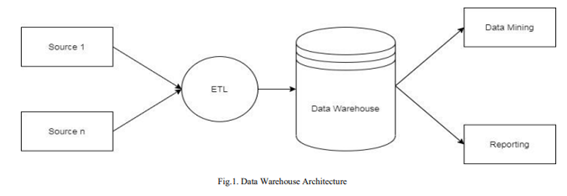
\includegraphics[width=7cm]{imagenes/imagen1.png}
\subsubsection{Ventajas de Data warehouse}

\begin{itemize}
    \item  Facilita la toma de decisiones basadas en datos, en cualquier área funcional de la empresa, ya que te proporciona información integrada y global del negocio.
    \item  La información se convierte en un valor añadido para cualquier negocio, gracias a que permite aplicar técnicas estadísticas de análisis y modelización que ayudan a encontrar relaciones ocultas entre los datos almacenados.
    \item Te permite de manera sencilla aprender de los datos del pasado y predecir situaciones futuras para diferentes escenarios.
    \item   Simplifica la implantación de sistemas de gestión integral de la relación con el cliente, dentro de la empresa.
    \item  Supone una optimización tecnológica y económica en entornos de Centro de Información, estadística o de generación de informes con retornos de la inversión espectaculares.
   \item Es un sistema especialmente útil para el medio y el largo plazo.
   \item Aumenta la productividad de las empresas de manera muy sustancial.
  \item Te permite realizar planes de una manera mucho más efectiva.
  \item Permite la integración de todas las herramientas corporativas. Por ejemplo, nosotros en Artyco integramos toda la información que recogemos a través de todas nuestras aplicaciones (monitorización web, crm, wifi tracking, campañas…) en un Data Warehouse, de donde sacar la información necesaria ante consultas determinadas.
  \item Para trabajar de manera correcta un Data Warehouse, es preciso que todos los componentes de la organización hablen el mismo lenguaje, es decir, que todos llamen a las cosas por su nombre. De este modo, gracias al Data Warehouse se pueden unificar conceptos. 
\end{itemize}


\subsection{DATA LAKE}
\subsubsection{Concepto}
El Data Lake es un repositorio compartido que le permite adquirir y almacenar grandes cantidades de datos procedentes de sistemas heterogéneos en formato nativo, es decir, datos en bruto estructurados, semiestructurados y no estructurados. La adquisición puede provenir de sistemas heredados, como CRM y ERP, o de fuentes externas, como feeds, Internet de las Cosas y datos de redes sociales.
El propósito de un Data Lake es, por lo tanto, proporcionar una visión no necesariamente refinada de los datos para apoyar las actividades de Data Discovery, lo que lo convierte en un sistema adecuado para usuarios expertos.
\includegraphics[width=7cm]{imagenes/imagen2.png}
\subsubsection{Atributos clave de un data lake}
\begin{itemize}
    \item  Cómputo y almacenamiento desacoplado.
    \item  Ingesta y transformación rápida.
    \item   Seguridad en ambientes multitenant
    \item   Query in place
    \item  Schema on read
\end{itemize}
Los data lakes extienden el enfoque tradicional al tener diversos motores de análisis, almacenamiento a bajo costo, escalas de TBs -EBs
\includegraphics[width=7cm]{imagenes/imagen3.png}
\subsubsection{Capas comunes de data lake(tecnologías)}
\begin{itemize}
    \item  Data Ingestion: capa temporal de carga en la que los datos pasan checks básicos antes de ser almacenados en la capa de raw data. Si bien no es necesaria, se puede implementar para llevar a cabo
    \item  controles básicos de calidad, como posibles filtros según el origen de los datos, descartando fuentes desconocidas
    \item  procesos de encriptación de los datos en caso de requerirse por motivos de seguridad
    \item  registros sencillos de metadata y trazabilidad mediante tags, almacenando el origen de los datos, fecha y hora de carga, el formato y otras características técnicas, su privacidad y nivel de seguridad, algoritmo de encriptación, etc.
    \item Data Storage (Raw Data): capa sin esquema establecido donde todos los datos, estructurados o no estructurados, son almacenados sin sufrir adaptaciones. Es una capa en la que se precisa de analistas expertos en data discovery mediante herramientas big data (Hive, Spark, Map Reduce…).
    \item  Data Processing (Zona de Confianza): Una vez que los analistas de datos han realizado data discovery en el raw data, se puede ver la necesidad de procesar y adaptar determinados sets de datos para alojarlos en una capa de uso recurrente. En esta capa pueden tener lugar procesos avanzados de data quality, integridad y otras adaptaciones para disponer de una capa de confianza de exploración de datos a la que tengan acceso otros usuarios.
    \item   Data Access (Zona de Consumo): esta es una capa más avanzada donde, finalmente, los datos se ponen a disposición de analistas de negocio. Estos analistas podrá generar informes y análisis para responder a preguntas de negocio y afianzar la toma de decisiones. 
\end{itemize}
\subsubsection{Arquitectura de Data lake}
\paragraph{Arquitectura de zona}
\begin{itemize}
    \item De estanque: Inmon diseña un lago de datos como un conjunto de estanques de datos [23]. un dato estanque se puede ver como una subdivisión de un lago de datos que trata con datos de un específico escribe. De acuerdo con las especificaciones de Dixon, cada estanque de datos está asociado con un sistema de almacenamiento especializado, algún procesamiento y acondicionamiento de datos específicos (es decir, transformación/preparación de datos) y un servicio de análisis relevante. Más precisamente, Inmon identifica cinco estanques de datos.
    \item  De zona : Arquitecturas de zona Las denominadas arquitecturas de zona asignan datos a una zona según a su grado de refinamiento.
\end{itemize}
\paragraph{Arquitecturas funcionales y de madurez}
Para superar las contradicciones de la categorización estanque/zona, se propone una forma alternativa de agrupar arquitecturas de lagos de datos con respecto al tipo de criterios Se utiliza para definir componentes. Como resultado, distinguimos arquitecturas funcionales, arquitecturas basadas en la madurez de datos y arquitecturas híbridas
\includegraphics[width=7cm]{imagenes/imagen4.png}
\subsubsection{Ventajas de Data lake}
\begin{itemize}
    \item El Data Lake permite centralizar todos los datos en un mismo lugar, vengan de la fuente que vengan. Una vez incluidas en su silo correspondiente de información, pueden ser procesadas a través de herramientas de Big Data. Muchas veces, en esa disparidad de información, habrá datos que requieran un tratamiento especial en cuanto a seguridad. Gracias al Data Lake, este aspecto se puede solventar.
    \item  Puede que la fuente original del dato esté obsoleta o se haya desactivado, sin embargo, su contenido puede que siga siendo valioso para el análisis. A través del Data Lake, puedes acceder a dicha información.
    \item  Todo dato que llegue al Data Lake puede ser normalizado y enriquecido.
    \item  Los datos se preparan en función de la necesidad del momento. Esto permite reducir considerablemente los costes y los tiempos. En el Data Warehouse, por ejemplo, es necesaria dicha preparación.
    \item  Se puede acceder a la información y enriquecerla desde cualquier punto del planeta, por cualquier usuario autorizado por el Data Lake. Esto ayuda a la organización a recopilar más fácilmente los datos necesarios para la toma de decisiones.
    \item  Un Data Lake pone la información en manos de un mayor número de personas dentro de cualquier organización, aprovechándose mejor la empresa de ese conocimiento que adquieren dichos individuos.
\end{itemize}
\subsection{Comparativa Data lake y Data Warehouse}
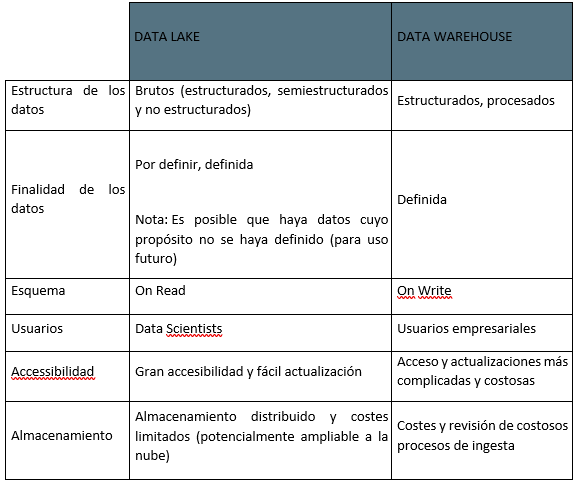
\includegraphics[width=7cm]{imagenes/imagen5.png}
\begin{itemize}
    \item  Los data lake y los data warehouse se utilizan de forma generalizada para el almacenaje de big data, pero, aunque ambos son almacenes de datos, estos no son términos intercambiables. Un data lake o "lago de datos" es un gran conjunto de datos en bruto, que todavía no tiene una finalidad definida. En cambio, un data warehouse o "almacén de datos" es un depósito de datos que ya están estructurados y filtrados y han sido procesados para un propósito concreto.
    \item   Datalake conserva todos los datos, a diferencia del almacén de datos, donde se dedica una parte importante de tiempo a decidir qué datos incluir y no incluir en el almacén.
    \item Data Lake admite todos los tipos de datos, independientemente de su tipo, formato o procedencia y sin necesidad de normalizar su estructura. La información se mantiene en su forma original y solo se transforma cuando se va a consumir.
    \item   Data Lake puede nutrir a todos los usuarios de la organización, incluyendo a esos perfiles técnicos con exigencias de análisis más avanzadas, que son quienes recurren a capacidades como análisis estadístico y modelado predictivo.
    \item   A diferencia del Data Warehouse, el Data Lake se adapta fácilmente a los cambios. El diseño del almacén es un proceso complejo y, la actualidad de loso negocios, en ocasiones no puede esperar tanto tiempo. Para esas circunstancias, asegura la adaptabilidad necesaria para entregar respuestas más rápidas.
\end{itemize}


\section{Conclusiones}

Es necesario revisar la categorías de un lago de datos y un almacén de datos, para analizar cual adapta mejor al caso de uso en el que se desea trabajar.
Cuando se construyen tuberías de datos, es necesario implementar una combinación de ambas soluciones de almacenamiento.


\section{Recomendaciones}
 El lago de datos integran diferentes tipos de datos para generar preguntas completamente nuevas, ya que es probable que estos usuarios no usen almacenes de datos porque pueden necesitar ir más allá de sus capacidades, mientras que en el almacén de datos la mayoría de los usuarios de una organización están operativos. Este tipo de usuarios solo se preocupa por los informes y las métricas clave de rendimiento.

 
 


%----------------------------------------------------------------------------------------
%	REFERENCE LIST
%----------------------------------------------------------------------------------------
\begin{thebibliography}{}

    \bibitem{DOC2008} 
    Data Lake vs Data Warehouse. Veamos sus principales diferencias. (2022). Powerdata.es. https://blog.powerdata.es/el-valor-de-la-gestion-de-datos/data-lake-vs-data-warehouse.-veamos-sus-principales-diferencias
    \bibitem{FRE2016} 
   Gorini, M. (2022). ¿Cuál es la diferencia entre un data lake y un data warehouse? Bismart.com. http://blog.bismart.com/diferencia-entre-data-lake-y-data-warehouse
	\bibitem{FRE2016} 
   Gigliotti, M. (2019). Data Lake y Data Warehouse: ¿Qué son y en qué se diferencian? Techedgegroup.com. https://www.techedgegroup.com/es/blog/data-lake-data-warehouse-definicion-diferencias
    \bibitem{FRE2019} 
   Data Lake vs Data Warehouse: Key Differences - Talend. (2022). Talend - a Leader in Data Integration Data Integrity. https://www.talend.com/resources/data-lake-vs-data-warehouse/
  
    \bibitem{FRE2019}
    Emilio Fernández Lastra. (2018, October 10). Data Warehouse y Data Lake. Qué son y para qué sirven. Artyco | the Data Driven Company. https://artyco.com/data-warehouse-data-lake-que-es/
    
    \bibitem{FRE2018}
   Prakash, S. S. (2020, April). Evolution of Data Warehouses to Data Lakes for Enterprise Business Intelligence. ResearchGate; unknown. https://www.researchgate.net/publication/343219651EvolutionofDataWarehousestoDataLakesforEnterpriseBusinessIntelligence/link/5f1d52ad92851cd5fa48958a/download
   
   \bibitem{FRE2018}
  Flores, A. (n.d.). Construyendo y governando Data Lakes y Data Warehouses modernos en AWS. Retrieved April 5, 2022, from https://d1.awsstatic.com/events/Summits/AMER2019/Mexico-City/BuildingandgoverningmoderndatalakesanddatawarehousesADB201.pdf
   
   \bibitem{FRE2018}
   Mendez, A., Britos, A.,  Garcia-Martínez, P. Y. (2003). Fundamentos de Data Warehouse. Reportes Técnicos En Ingeniería Del Software, 5(1), 19–26. http://artemisa.unicauca.edu.co/~ecaldon/docs/bd/fundamentosdedatawarehouse.pdf
    
    \bibitem{FRE2018}
    Agudelo, J. (2020) Data Lakes: Aplicaciones, Herramientas y Arquitecturas. Monografía presentada como requisito para optar al Título de Ingeniero de Sistemas y Computación https://repositorio.utp.edu.co/server/api/core/bitstreams/5f56e572-d416-487e-a6d5-ec3a8e45da46/content
 
	\bibitem{FRE2018}
	Pegdwendé Sawadogo, Jérôme Darmont. On data lake architectures and metadata management. Journal of Intelligent Information Systems, Springer Verlag, 2021, 56 (1), pp.97-120. ff10.1007/s10844- 020-00608-7ff. ffhal-03114365f https://hal.archives-ouvertes.fr/hal-03114365/document


 
    \end{thebibliography}


%----------------------------------------------------------------------------------------

\end{document}